\chapter{Momentum}

\section{momentum \& momentum conservation}

\subsection{momentum}

\begin{ilight}
	\centering \keypoint{momentum} of an object is defined as the product of its mass and its velocity: \begin{empheq}[box=\tcbhighmath]{equation*}{p=mv}\end{empheq} \index{momentum}
\end{ilight}

\cmt unit of momentum: $[p]=\text{kg m s}^{-1} = \text{N s}$

\cmt momentum is a vector quantity

momentum is in same direction as the object's velocity

to find change in momentum of a body, or to find sum of the momenta\footnote{Momenta is the plural form of momentum.} for a system of several objects, one has to keep track of directions

\cmt momentum is like inertia in motion

inertia, the property that object resists change in motion, is incorporated in Newton's first law

we will see very soon that momentum is closely related to Newton's second law

\subsection{relation to force}

suppose a constant net force $F$ is applied on a body, we can write:
\begin{equation*}
	F = ma = m\frac{\Delta v}{\Delta t} = \frac{m\Delta v}{\Delta t} = \frac{\Delta p}{\Delta t}
\end{equation*}
where we have used Newton's second law and defining equation for momentum

from this derivation, we can give a formal definition for the force

\begin{ilight}
	\centering \keypoint{force} is defined as the rate of change in momentum: \begin{empheq}[box=\tcbhighmath]{equation*}{F = \frac{\Delta p}{\Delta t}}\end{empheq}\index{force}
\end{ilight}

we can also restate Newton's second law in terms of momentum:

\begin{ilight}
	\keypoint{Newton's second law} states that resultant force acting on an object equals the rate of change in the object's momentum
\end{ilight}

\cmt information about force can be extracted from momentum-time graphs

{
	\centering
	
	\begin{empheq}[box=\tcbhighmath]{equation*}{ \text{gradient of } p\text{-}t \text{ graph equals the resultant force acting} }\end{empheq}
	
}

\cmt information about \emph{change} in momentum can be deduce from force-time graphs
	
{
	\centering

	\begin{empheq}[box=\tcbhighmath]{equation*}{ \text{area under } F\text{-}t \text{ graph equals the change in object's momentum} }\end{empheq}
	
}

\example{A ball of 120 g strikes a wall at right angle with a speed of $10 \mps$. It rebounds with the same speed. If the time of impact is 25 ms, find the average force exerted on the ball.}

\begin{soln} change in momentum: $\Delta p = mv - mu = 0.12 \times 10 - 0.12 \times (-10) = 2.4 \text{ kg m s}^{-1}$

average force: $F=\frac{\Delta p}{\Delta t} = \frac{2.4}{2.5 \times10^{-3}} = 96 \text{ N}$ \end{soln}

\example{Water is pumped through a hose-pipe. A man is holding the hose-pipe horizontally and water emerges from the hose-pipe with a speed of $16\mps$ at a rate of 45 kg per minute. Find the force required from this man to hold steady the hose-pipe.}

\begin{soln}
\begin{equation*}
	F = \frac{\Delta p}{\Delta t} = \frac{\Delta (mv)}{\Delta t} = \frac{\Delta m (v-0)}{\Delta t} = \frac{45 \times 16}{60} \RA F = 12\text{ N} 
\end{equation*}
\end{soln}

\example{A strong wind of speed $30\mps$ blows against a wall of area 10 m$^2$ at right angles. The density of the air is 1.2 kg m$^{-3}$. Assume air speed reduces to zero when it hits the wall. What is the approximate force exerted by the air on the wall?}

\begin{soln}

{
	\centering
	
	$ F = \frac{\Delta p}{\Delta t} = \frac{\Delta (mv)}{\Delta t} = \frac{\Delta m (v-0)}{\Delta t} \xlongequal{m=\rho V} \frac{\rho \Delta V v}{\Delta t} \xlongequal{V=AL} \frac{\rho A \Delta L v}{\Delta t} \xlongequal{\Delta L = v \Delta t} \rho A v^2 $
	\eqyskip\begin{equation*}
	\RA F = 1.2 \times 10 \times 30^2 = 10800 \text{ N} 
	\end{equation*}
	
}
\end{soln}

\example{Given the variation with time of the momentum of a body as shown in the $p$-$t$ graph, check yourself that the variation of force acting and the variation of the object's acceleration should be plotted as shown in the $F$-$t$ graph and the $a$-$t$ graph.}


\begin{figure*}[ht]
	\centering
	\begin{minipage}{0.32\textwidth}
		\centering
		\begin{tikzpicture}
		\draw[<->] (0,3) node[left]{$p$} -- (0,0) -- (4,0) node[below]{$t$};
		\draw[thick,blue] (0,0) parabola[bend at end] (1.2,1) -- (2.4,1) parabola (3.6,2.7);
		\draw[dashed] (1.2,0) node[below]{$t_1$} -- (1.2,1) (2.4,0) node[below]{$t_2$} -- (2.4,1);
		\end{tikzpicture}
	\end{minipage}\hfil
	\begin{minipage}{0.32\textwidth}
		\centering
		\begin{tikzpicture}
		\draw[<->] (0,3) node[left]{$F$} -- (0,0) -- (4,0) node[below]{$t$};
		\draw[thick,red] (0,1.4) -- (1.2,0) -- (2.4,0) -- (3.6,1.4*1.7);
		\draw[dashed] (1.2,0) node[below]{$t_1$} (2.4,0) node[below]{$t_2$} ;
		\end{tikzpicture}
	\end{minipage}\hfil
	\begin{minipage}{0.32\textwidth}
		\centering
		\begin{tikzpicture}
		\draw[<->] (0,3) node[left]{$a$} -- (0,0) -- (4,0) node[below]{$t$};
		\draw[thick,red] (0,1.4) -- (1.2,0) -- (2.4,0) -- (3.6,1.4*1.7);
		\draw[dashed] (1.2,0) node[below]{$t_1$} (2.4,0) node[below]{$t_2$} ;
		\end{tikzpicture}
	\end{minipage}
\end{figure*}



\newpage

\begin{marginfigure}
	\vspace*{4pt}
	\centering
	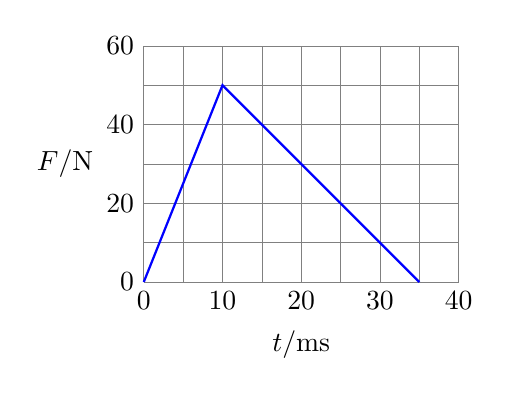
\begin{tikzpicture}
	\draw[step=0.5,thin,gray!50,help lines] (0,0) grid (4,3);
	\foreach \x/\xlabel in {0/0,1/10,2/20,3/30,4/40} \node[below] at (\x,0) {$\xlabel$};
	\foreach \y/\ylabel in {0/0,1/20,2/40,3/60} \node[left] at (0,\y) {$\ylabel$};
	\node at (2,-0.8) {$t$/ms};
	\node at (-1.0,1.5) {$F$/N};
	\draw[thick,blue] (0,0) -- (1,2.5) -- (3.5,0);
	\end{tikzpicture}
	\vspace*{-16pt}
\end{marginfigure}

\example{An object of mass 70 g is initially at rest. A force that varies with time is exerted on the object. The graph shows the how the force varies during the time of impact. What is the final velocity of the object?}

\begin{soln} area under $F$-$t$ graph gives change in momentum

{
	\centering
	
	$ \Delta p = \frac{1}{2} \times 50 \times 35\times10^{-3} = 0.875 \text{ kg m s}^{-1} $
	
}

final velocity: $v = \frac{\Delta p}{m} = \frac{0.875}{70\times10^{-3}} = 12.5 \mps $ \end{soln}


\subsection{Impulse-momentum relation}

we can further introduce a quantity called the impulse\footnote{The notion of impulse is not required by the AS Physics syllabus.}

\keypoint{impulse} is defined as the product of a force and time interval at which it acts: $J = F \Delta t$

$F\Delta t$ gives change in momentum, therefore we have the  impulse-momentum relation: $J=\Delta p$\index{momentum!impulse-momentum relation}

\cmt impulse-momentum relation is just another way of expressing Newton's second law

but the idea of impulse and momentum allows analysis of variable mass




\subsection{principle of momentum conservation}\label{ch:momentum-conservation}

change in an object's momentum is given by: $\Delta p = F \Delta t$
\footnote{The relation $\Delta p = F \Delta t$ is valid if we are dealing with a \emph{constant} force. If the object is acted by a varying force, then the change in its momentum is given by: $\Delta p = \int F \dd t$.}

in particular, if there is zero net force, then object's momentum stays constant

%\vspace*{\baselineskip}

this idea can be generalised to a system of objects

there are external forces from outside and internal forces between objects within the system

let's take two mutually interacting objects within the system, say $A$ and $B$

by Newton's 3rd law, force on $A$ by $B$ is equal and opposite to force on $B$ by $A$

change in $A$'s momentum by $B$ is then equal and opposite to change in $B$'s momentum by $A$

change in total momentum of $A$ and $B$ due to each other is therefore cancelled out

therefore, for the system as a whole, effect of internal forces always cancel out

change of total momentum of the system would only depend on net external force
\sidenote[][-6cm]{A more rigorous derivation goes as follows.
	
	Let's consider a system of point objects $m_i$, each experiences a resultant force $F_i$ where $F_i$ can come from some external source or another object $j$ within the system: $F_i = F_{i,\text{ext}} + \sum_j F_{i,j}$.
	
	Summing over all objects, we can write: $\sum_i F_i = \sum_i F_{i,\text{ext}} + \sum_{i,j} F_{i,j}$ 
	
	For each pair $i$ and $j$, the action-reaction principle suggests that the mutual interaction between the two are equal but opposite: $F_{i,j} = -F_{j,i}$, so $\sum_{i,j} F_{i,j} = 0$. Therefore, $\sum_i F_i = \sum_i F_{i,\text{ext}}$.
	
	Multiply both sides by $\Delta t$, we can write: $\sum_i F_i \Delta t = \sum_i F_{i,\text{ext}} \Delta t$. Note that $\sum_i F_i \Delta t = \sum_i \Delta p_i$ gives the change in total momentum of system, so this shows the change of total momentum is determined by the net external force: \begin{empheq}[box=\tcbhighmath]{equation*}{\left(\sum_i F_{i,\text{ext}} \right)\Delta t = \sum_i \Delta p_i}\end{empheq}}


if there is no net external force, then no change in total momentum

\begin{ilight}
	for any closed system where net external force is zero, the total momentum of the system remains constant, this is called the \keypoint{principle of momentum conservation} \index{conservation of momentum}
\end{ilight}

\example{A uranium-238 nucleus disintegrates, emitting an $\alpha$-particle of mass 4u and producing a thorium-234 nucleus of mass 234u. The uranium nucleus is initially at rest. (a) What is the ratio of the velocities of the product particles $\frac{v_\alpha}{v_\text{Th}}$?} (b) Explain why the $\alpha$-particle and the thorium nucleus must be emitted in opposite directions.

\begin{soln}
    
 no external force involved during decay, so momentum is conserved

zero initial momentum means total momentum of $\alpha$-particle and thorium nucleus is zero

$\alpha$-particle and thorium nucleus must carry equal but opposite momenta

equal momentum $\RA m_\alpha v_\alpha = m_\text{Th} v_\text{Th} \RA \frac{v_\alpha}{v_\text{Th}} = \frac{m_\text{Th}}{m_\alpha} = \frac{234}{4}=58.5 $

opposite momentum so they move off in exactly opposite directions \end{soln}



\subsection{collision problems}


for two bodies colliding together, external forces are negligible during the time of contact

hence total momentum is considered to be conserved for any collision process

\subsection{collision in one dimension}

suppose two masses $m_1$ and $m_2$ are restricted to move in one dimension only

they move at initial velocities $u_1$ and $u_2$ before they collide

after collision, their velocities become $v_1$ and $v_2$, as depicted in the diagram

\begin{figure}[!ht]
\centering
\begin{minipage}{0.45\textwidth}
	\begin{center}
		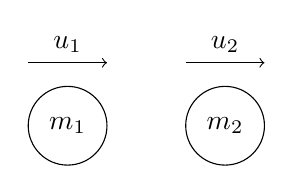
\begin{tikzpicture}
		\draw (-1,0) circle (0.5) node{$m_1$};
		\draw (1,0) circle (0.5) node{$m_2$};
		\draw[->] (-1.5,.8) -- (-0.5,.8) node[midway,above]{$u_1$};
		\draw[->] (0.5,.8) -- (1.5,.8) node[midway,above]{$u_2$};
		\end{tikzpicture}
		
		before collision
	\end{center}
\end{minipage}\hfil
\begin{minipage}{0.45\textwidth}
	\begin{center}
		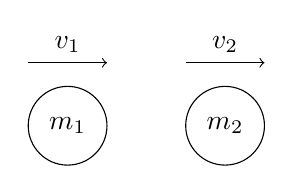
\begin{tikzpicture}
		\draw (-1,0) circle (0.5) node{$m_1$};
		\draw (1,0) circle (0.5) node{$m_2$};
		\draw[->] (-1.5,.8) -- (-0.5,.8) node[midway,above]{$v_1$};
		\draw[->] (0.5,.8) -- (1.5,.8) node[midway,above]{$v_2$};
		\end{tikzpicture}
		
		after collision
	\end{center}
\end{minipage}
\end{figure}

\rcyskip
total momentum is conserved, so: \begin{empheq}[box=\tcbhighmath]{equation*}{m_1 u_1 + m_2 u_2 = m_1 v_1 + m_2 v_2} \end{empheq}

\cmt recall the vector nature of momentum and velocity

we normally choose objects moving to the right to have positive momentum/velocity

then object travelling to the left would have negative momentum/velocity

\begin{marginfigure}
	\vspace*{-12pt}
	\centering
	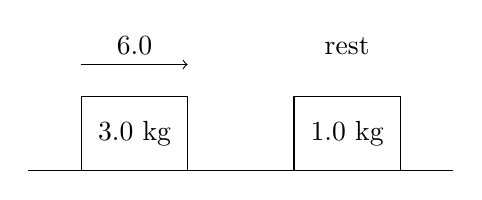
\begin{tikzpicture}[scale=1.35]
	\draw (-2,0) -- (2,0);
	\draw (-1.5,0) rectangle (-0.5,0.7) (-1,0.35) node{3.0 kg};
	\draw (0.5,0) rectangle (1.5,0.7) (1,0.35) node{1.0 kg};
	\draw[->] (-1.5,1) -- (-0.5,1) node[midway,above]{$6.0\mps$};
	\draw (1,1) node[above]{rest};
	\end{tikzpicture}
	\vspace*{-16pt}
\end{marginfigure}

\example{A 3.0 kg mass moving at $6.0 \mps$ has a head-on collision with a stationary 1.0 kg mass. The two masses stick together on impact. What is the final velocity of the two masses?}

\begin{soln}\begin{equation*}
	m_1 u_1 + \cancelto{0}{m_2 u_2} = (m_1+m_2)v \RA 3.0\times6.0 = (3.0+1.0)\times v 
 \end{equation*}
 \begin{equation*}
 \RA v=4.5 \mps 
\end{equation*}
\end{soln}
\begin{marginfigure}
	\vspace*{6pt}
	\centering
	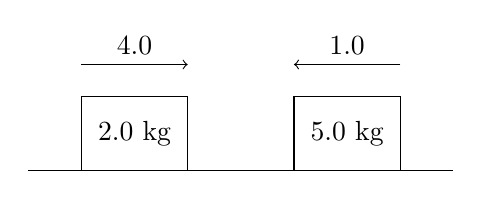
\begin{tikzpicture}[scale=1.35]
	\draw (-2,0) -- (2,0);
	\draw (-1.5,0) rectangle (-0.5,0.7) (-1,0.35) node{2.0 kg};
	\draw (0.5,0) rectangle (1.5,0.7) (1,0.35) node{5.0 kg};
	\draw[->] (-1.5,1) -- (-0.5,1) node[midway,above]{$4.0\mps$};
	\draw[->] (1.5,1) -- (0.5,1) node[midway,above]{$1.0\mps$};
	\end{tikzpicture}
	\vspace*{-16pt}
\end{marginfigure}

\example{A 2.0 kg mass moving at $4.0 \mps$ collides head on with a 5.0 kg mass moving at $1.0 \mps$. After the collision, speed of the 5.0 kg mass is unchanged but its direction is reversed. What is the velocity of the 2.0 kg mass after the collision?}

\begin{soln}\begin{equation*}
m_1 u_1 + m_2 u_2 = m_1 v_1 + m_2 v_2 \, 
\end{equation*}
\begin{equation*}
\ra \, 2.0\times4.0+5.0\times(-1.0) = 2.0 \times v_1 + 5.0\times1.0 \, \ra \,  v_1 = -1.0 \mps
\end{equation*}

minus sign means the 2.0 kg mass reverses direction after collision \end{soln}

\subsection{elastic \& inelastic collisions}

\subsection*{elastic collisions}

collision can be either elastic or inelastic\footnote{Here we assume you already have some knowledge about \emph{kinetic energy}. Kinetic energy of a moving body is given by the formula: $E_k = \frac{1}{2}mv^2$. You might have learned about it in an GCSE course or elsewhere. We will talk about kinetic energy in \S\ref{ch-KE}.}

\begin{ilight}
	for \keypoint{elastic collisions}, there is no loss of kinetic energy
\end{ilight}



we hereby derive a condition that must be satisfied by two objects colliding elastically

since momentum and kinetic energy are both conserved, we can write two equations\footnote{For simplicity, we consider two-body collision in one dimension only, that is the two bodies move along the same straight line before and after the collision. For a two-body collision problem in two dimension, the conservation of momentum can be broken into two independent component equations.}
\begin{gather*}
	{ m_1 u_1 + m_2 u_2 = m_1 v_1 + m_2 v_2 }\\
	{ \frac{1}{2}m_1 u_1^2 + \frac{1}{2}m_2 u_2^2 = \frac{1}{2}m_1 v_1^2 + \frac{1}{2}m_2 v_2^2  }
\end{gather*}

rearranging both equations, we have
\begin{gather}
m_1 (u_1 - v_1) = m_2 (v_2 - u_2) \tag{1}\\
m_1 (u_1^2 - v_1^2) = m_2 (v_2^2 - u_2^2)  \tag{2}
\end{gather}

equation (4) can be further rewritten as
\begin{equation*}
	m_1 (u_1 - v_1)(u_1 + v_1) = m_2 (v_2 - u_2)(v_2 + u_2) \tag{2'}
\end{equation*}

comparing equation (2') to equation (1), one has: $u_1 + v_1 = v_2 + u_2$

rearrange the equation, we find: $ \boxed{v_2 - v_1 = u_1 - u_2} $

both side of the equation now represent a \emph{relative speed} between the two colliding bodies

\begin{ilight}
for an elastic collision process between two bodies, the relative velocity of separation after collision equals the relative velocity of approach before collision
\end{ilight}

\subsection*{inelastic collisions}

\begin{ilight}
	for \keypoint{inelastic collisions}, part of kinetic energy is lost due to change in object's shape
\end{ilight}

\cmt for an inelastic process, the following will hold:

\titem K.E. after collision is less than K.E. before collision

\titem relative speed after collision is less than relative speed before collision



\subsection*{brief summary}

discussions on elastic and inelastic collisions are summarised in the table below

\begin{center}
	\begin{tabular}{|c|c|c|}
		\hline  & elastic collision & inelastic collision \\ 
		\hline conservation of momentum  & \ding{51} & \ding{51} \\ 
		\hline conservation of kinetic energy & \ding{51} & \ding{55} \\
		\hline conservation of total energy & \ding{51} & \ding{51} \\ 
		\hline relative speed stays unchanged & \ding{51} & \ding{55} \\ 
		\hline 
	\end{tabular} 
\end{center}



\example{A sphere of mass $m$ moves on a smooth horizontal surface at speed $v$ and collides \emph{elastically} with an identical ball at rest. What are the final velocities of the two spheres?}

\begin{figure}[!ht]
	\centering
	\begin{minipage}{0.45\textwidth}
		\begin{center}
			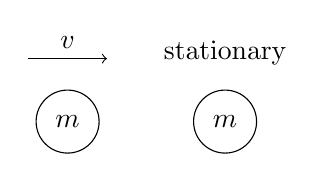
\begin{tikzpicture}
			\draw (-1,0) circle (0.4) node{$m$};
			\draw (1,0) circle (0.4) node{$m$};
			\draw[->] (-1.5,.8) -- (-0.5,.8) node[midway,above]{$v$};
			\draw (1,.6) node[above]{stationary};
			\end{tikzpicture}
			
			before collision
		\end{center}
	\end{minipage}\hfil
	\begin{minipage}{0.45\textwidth}
		\begin{center}
			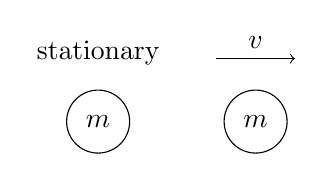
\begin{tikzpicture}
			\draw (-1,0) circle (0.4) node{$m$};
			\draw (1,0) circle (0.4) node{$m$};
			\draw (-1,.6) node[above]{stationary};
			\draw[->] (0.5,.8) -- (1.5,.8) node[midway,above]{$v$};
			\end{tikzpicture}
			
			after collision
		\end{center}
	\end{minipage}	
\end{figure}

\begin{soln}
\begin{equation*}
\begin{array}{ll}
mv = mv_1 + mv_2 & \text{(momentum conservation)}\\
v = v_2 - v_1 & \text{(relative speed unchanged)} \end{array} 
\RA
\Bigg\{
\begin{array}{ccc}
v_1 &=& 0 \\
v_2 &=& v
\end{array}
\end{equation*}

the two spheres simply exchange velocities during the collision, as shown in diagram \end{soln}\sidenote{If two objects of equal mass collide elastically with one another, one can actually show that their velocities would exchange regardless of their initial velocities.}

\example{A 4.2 kg mass $A$ and a 1.5 kg mass $B$ are travelling towards each other on a frictionless horizontal plane. Mass $A$ and $B$ move at $5.40\mps$ and $1.80\mps$ respectively before they strike, as shown below. Mass $B$ moves to the right at $4.50\mps$ after the collision, (a) find the velocity of $A$ after the impact, and (b) suggest whether the collision is elastic.}

\begin{figure}[ht]
	\centering
	\begin{minipage}{0.45\textwidth}
		\centering
		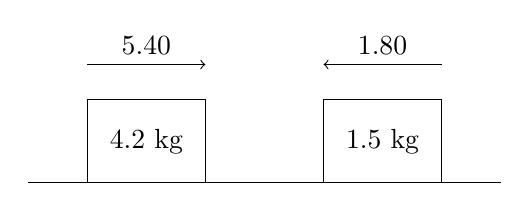
\begin{tikzpicture}[scale=1.5]
		\draw (-2,0) -- (2,0);
		\draw (-1.5,0) rectangle (-0.5,0.7) (-1,0.35) node{4.2 kg};
		\draw (0.5,0) rectangle (1.5,0.7) (1,0.35) node{1.5 kg};
		\draw[->] (-1.5,1) -- (-0.5,1) node[midway,above]{$5.40\mps$};
		\draw[->] (1.5,1) -- (0.5,1) node[midway,above]{$1.80\mps$};
		\end{tikzpicture}
		
		before collision
	\end{minipage}\hfil
	\begin{minipage}{0.45\textwidth}
		\centering
		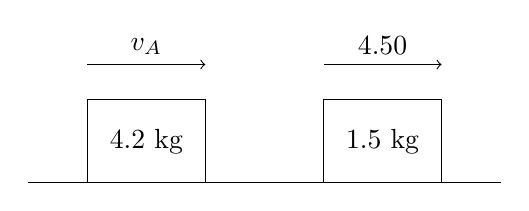
\begin{tikzpicture}[scale=1.5]
		\draw (-2,0) -- (2,0);
		\draw (-1.5,0) rectangle (-0.5,0.7) (-1,0.35) node{4.2 kg};
		\draw (0.5,0) rectangle (1.5,0.7) (1,0.35) node{1.5 kg};
		\draw[->] (-1.5,1) -- (-0.5,1) node[midway,above]{$v_A$};
		\draw[<-] (1.5,1) -- (0.5,1) node[midway,above]{$4.50\mps$};
		\end{tikzpicture}
		
		after collision
	\end{minipage}
\end{figure}

\begin{soln} momentum conserved: $m_A u_A + m_B u_B = m_A v_A + m_B v_B$

{
	\centering
	
	$ 4.2\times5.40 + 1.5\times(-1.80) = 4.2\times v + 1.5\times4.50 \RA v_A = 3.15 \mps$
	
}

K.E. before: $ E_{k,i} = \frac{1}{2}m_A u_A^2 + \frac{1}{2}m_A u_B^2 = \frac{1}{2}\times4.2\times5.40^2 + \frac{1}{2}\times1.5\times1.80^2 \approx 63.7 \text{ J}$

\eqyskip K.E. after: $ E_{k,f} = \frac{1}{2}m_A v_A^2 + \frac{1}{2}m_A v_B^2 = \frac{1}{2}\times4.2\times3.15^2 + \frac{1}{2}\times1.5\times4.50^2 \approx 36.0 \text{ J}$

there is K.E. loss, so collision is inelastic

alternatively, we can compare the relative speed before and after the collision

{
	\centering
	
	$ u_A - u_B = 5.40 - (-1.80) = 7.20 \mps \qquad v_B - v_A = 4.50 - 3.15 = 1.35 \mps$
	
}

relative speed changed after the collision, so collision must be inelastic \end{soln}


\subsection{collision in two dimensions}

when objects collide on a horizontal plane, they can possibly move off in any direction

negligible net external force is present, total momentum is still conserved

recall that momentum is a vector quantity, so momentum should be conserved in any direction

\vspace*{\baselineskip}

let's consider the collision between two masses $m_1$ and $m_2$

for simplicity, assume their initial velocities $u_1$ and $u_2$ are in same direction

final velocities $v_1$ and $v_2$ after the collision are shown

\begin{figure}[!ht]
	\centering
	\begin{minipage}{0.32\textwidth}
		\begin{center}
			\begin{tikzpicture}
			\draw[white] (0,-3) -- (0,2)node[left]{$y$};
			\draw (-1.2,0) circle (0.3) node{$m_1$};
			\draw (1.2,0) circle (0.3) node{$m_2$};
			\draw[blue,thick,->] (-0.9,0) --++ (1,0) node[midway,above]{$u_1$};
			\draw[blue,thick,->] (1.5,0) --++ (1,0) node[midway,above]{$u_2$};
			\end{tikzpicture}
			
			before collision
		\end{center}
	\end{minipage}\hfil
	\begin{minipage}{0.32\textwidth}
		\begin{center}
			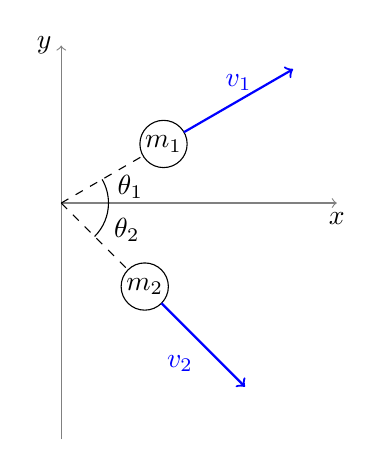
\begin{tikzpicture}
			\draw[gray,->] (0,-3) -- (0,2) node[left,black]{$y$};
			\draw[gray,->] (0,0) -- (3.5,0) node[below,black]{$x$};
			\draw[fill=white] (30:1.5) circle (0.3) node{$m_1$};
			\draw[fill=white] (-45:1.5) circle (0.3) node{$m_2$};
			\draw[blue,thick,->] (30:1.8) --++ (30:1.6) node[midway,above]{$v_1$};
			\draw[blue,thick,->] (-45:1.8) --++ (-45:1.5) node[midway,below left]{$v_2$};
			\draw[dashed] (0,0) -- (30:1.2);
			\draw[dashed] (0,0) -- (-45:1.2);
			\draw (0.6,0) arc (0:30:0.6) (13:0.9) node {$\theta_1$};
			\draw (0.6,0) arc (0:-45:0.6) (-22:0.9) node {$\theta_2$};
			\end{tikzpicture}
			
			after collision
		\end{center}
	\end{minipage}\hfil
	\begin{minipage}{0.32\textwidth}
	\begin{center}
		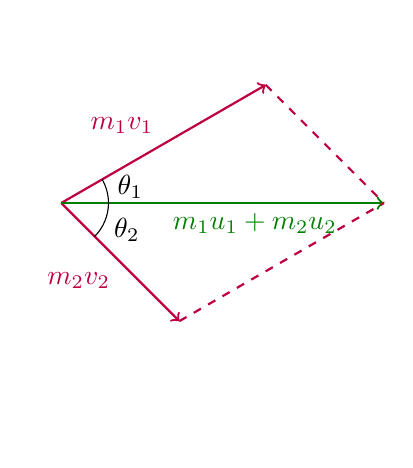
\begin{tikzpicture}
		\draw[white] (0,-3) -- (0,2)node[left]{$y$};
		\draw[thick,purple,->] (0,0) -- (30:3) node[midway,above left]{$m_1 v_1$};
		\draw[thick,purple,->] (0,0) --++ (-45:{1.5*sqrt(2)}) node[midway,below left]{$m_2 v_2$};
		\draw[thick,Green,->] (0,0) --++ ({1.5*sqrt(3)+1.5},0) node[pos=0.6,below]{$m_1 u_1 + m_2 u_2$};
		\draw (0.6,0) arc (0:30:0.6) (13:0.9) node {$\theta_1$};
		\draw (0.6,0) arc (0:-45:0.6) (-22:0.9) node {$\theta_2$};
		\draw[thick,purple,dashed] (-45:{1.5*sqrt(2)}) --++ (30:3);
		\draw[thick,purple,dashed] (30:3) --++ (-45:{1.5*sqrt(2)});
		\end{tikzpicture}
	
	momentum conservation
\end{center}
\end{minipage}
\end{figure}

equations of momentum conservation can be written for two perpendicular directions
\begin{equation*}
	\begin{array}{rcll}
	m_1 u_1 + m_2 u_2 &=& m_1 v_1 \cos\theta_1 + m_2 v_2 \cos\theta_2 & \qquad (\text{in }x\text{-direction}) \\
	0 &=& m_1 v_1 \sin\theta_1 - m_2 v_2 \sin\theta_2  & \qquad (\text{in }y\text{-direction}) \end{array}
\end{equation*}

\eqyskip one can also construct a vector triangle to transform the problem into a geometry problem

\begin{figure}
\centering
\begin{minipage}{0.22\textwidth}
	\begin{center}
		\begin{tikzpicture}[scale=0.96]
			\draw[white] (0,1) ++ (60:0.4) --++ (60:1.5);
			\draw[white] (0,-1) ++ (-30:0.4) --++ (-30:1.5) node[midway,below left]{$v_2$};;
			\draw (-.8,0) circle (0.4) node{$m_1$};
			\draw (.8,0) circle (0.4) node{$m_2$};
			\draw[->] (-1.3,.8) -- (-0.3,.8) node[midway,above]{$u$};
			\node[above] at (.8,0.7) {rest};
		\end{tikzpicture}
			
			before collision
	\end{center}
\end{minipage}
\begin{minipage}{0.22\textwidth}
	\begin{center}
		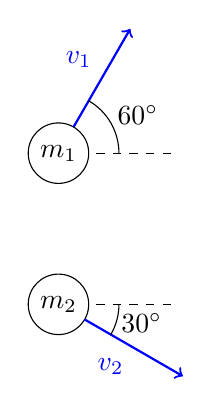
\begin{tikzpicture}[scale=0.96]
			\draw (0,1) circle (0.4) node{$m_1$};
			\draw (0,-1) circle (0.4) node{$m_2$};
			\draw[->,blue,thick] (0,1) ++ (60:0.4) --++ (60:1.5) node[midway,above left]{$v_1$};
			\draw[->,blue,thick] (0,-1) ++ (-30:0.4) --++ (-30:1.5) node[midway,below left]{$v_2$};
			\draw[dashed] (0.5,1) --++ (1,0);
			\draw (.8,1) arc(0:60:.8);
			\node at (1.05,1.5) {$60^\circ$};
			\draw[dashed] (0.5,-1) --++ (1,0);
			\draw (.8,-1) arc(0:-30:.8);
			\node at (1.1,-1.25) {$30^\circ$};
		\end{tikzpicture}
			
		after collision
	\end{center}
\end{minipage}

\vspace*{1.35\baselineskip}

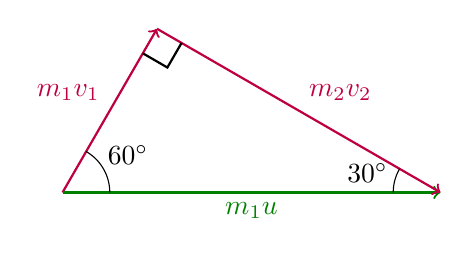
\begin{tikzpicture}[scale=1.2]
\draw[thick,purple,->] (0,0) --++ (60:2) node[midway, above left]{$m_1v_1$};
\draw[thick,Green,->] (0,0) --++ (0:4) node[midway, below]{$m_1 u$};;
\draw[thick,purple,->] (60:2) -- (0:4) node[midway, above right]{$m_2v_2$};
\draw[thick] (60:1.7) --++ (-30:0.3) --++ (60:0.3);
\draw (0.5,0) arc(0:60:0.5);
\draw (30:0.8) node {$60^\circ$};
\draw (3.5,0) arc(180:150:0.5);
\draw (4,0) ++ (165:0.8) node {$30^\circ$};
\end{tikzpicture}
\end{figure}

\example{A ball of mass $m_1 = 1.0 \text{ kg}$ travelling with a speed of $u=6.0 \mps$ in the $x$-direction strikes a stationary ball of mass $m_2 = 2.0 \text{ kg}$. The direction of the balls' velocities $v_1$ and $v_2$ after the collision are shown in the diagram. Find $v_1$ and $v_2$.}

\begin{soln} start with momentum conservation equations:

\eqskip$\left\{\begin{array}{l}
	m_1 u = m_1 v_1 \cos60^\circ + m_2 v_2 \cos30^\circ \\
	0 = m_1 v_1 \sin60^\circ - m_2 v_2 \sin30^\circ
	\end{array} \right. $

\eqskip $ \left\{\begin{array}{l}
	1.0\times6.0 = 1.0 \times v_1 \times \frac{1}{2} + 2.0 \times v_2 \times \frac{\sqrt{3}}{2}  \\
	0 = 1.0 \times v_1 \times \frac{\sqrt{3}}{2} - 2.0 \times v_2 \times \frac{1}{2}
	\end{array} \right. $

\eqyskip simplify and solve the equations:

\eqskip $ \left\{\begin{array}{l}
\frac{1}{2} v_1 + \sqrt{3} v_2 = 6 \\
v_2 =  \frac{\sqrt{3}}{2} v_1
\end{array} \right. \RA 
\left\{\begin{array}{l}
v_1 = 3.0 \mps \\
v_2 \approx 2.6 \mps
\end{array} \right.$

\eqyskip one can also draw and use the vector triangle

for this question, this happens to be a right-angled triangle, so things become much easier
\begin{equation*}
	\left\{\begin{array}{l}
	m_1 v_1 = m_1 u \cos 60^\circ \\
	m_2 v_2 = m_1 u \cos 30^\circ
	\end{array} \right. \RA 
	\left\{\begin{array}{l}
	1.0\times v_1 = 1.0 \times 6.0 \times \frac{1}{2} \\
	2.0\times v_2 = 1.0 \times 6.0 \times \frac{\sqrt{3}}{2}
	\end{array} \right.	\RA 
\end{equation*}
\begin{equation*}
	\left\{\begin{array}{l}
	v_1 = 3.0 \mps \\
	v_2 \approx 2.6 \mps
	\end{array} \right.  
\end{equation*}
\end{soln}



\subsection{end-of-chapter questions}
	
From this definition, we see that the force acting depends on the magnitude of the change in momentum, but also depends on how long this change occurs. , it would be silly to land on the ground with stiff legs. You naturally bend your knees. Acrobats in a circus fall on a soft mat or a safety net. All these actions does not change the impulse, but they increase the time of contact, and therefore reduce the force that might cause harmful injuries.


\subsection*{force \& momentum}

\question{When speed cars run out of control in a racing game, why are they stopped by haystacks instead of concrete walls? When you jump from an elevated position and land on the ground, you naturally bend your knees instead of keeping your legs stiff. How does that reduce the chance of causing harmful injuries?}
	
\question{Automobiles were manufactured to be as rigid as possible, but nowadays many cars are designed to crumple upon impact. Can you explain why?}

\subsection*{principle of momentum conservation}

\question{How does conservation of momentum apply to a ball bouncing off a wall?}

\question{In the comic hero series, Superman hurls an asteroid in outer space, and he is seen at rest after the throw. What law of physics is violated here? If the asteroid is 100 times as massive as the superhero, and it is thrown at $50\mps$. What is Superman's velocity right after the throw?}



\subsection*{collision problems}

\question{When a piece of putty falls and hits the floor without bouncing, what becomes of its momentum before impact? What becomes of its kinetic energy?}
	

